\section{Planning}

$ \ast $ \textit{La section suivante pourra être négocié de manière à ce que toutes les parties prenantes soient en accord avec le contenu.} \\

Durant ce projet, plusieurs types de livrables seront remis au client, tel que les comptes-rendus de réunion, les soutenances, ou d’autres documents de suivi. Afin de clarifier certains points d’interrogation et de rendre compte de l’avancement du projet. Par ailleurs, il existe également les livrables produits, qui correspondent aux différentes composantes du produit à rendre out au long de la phase de développement, ou au produit final lui-même à rendre à la fin du projet. \\[2em]


Le diagramme de Gantt ci-dessous permet de visualiser les livrables, produits à rendre au clients.
\begin{figure}[h]
   \centering
   {
      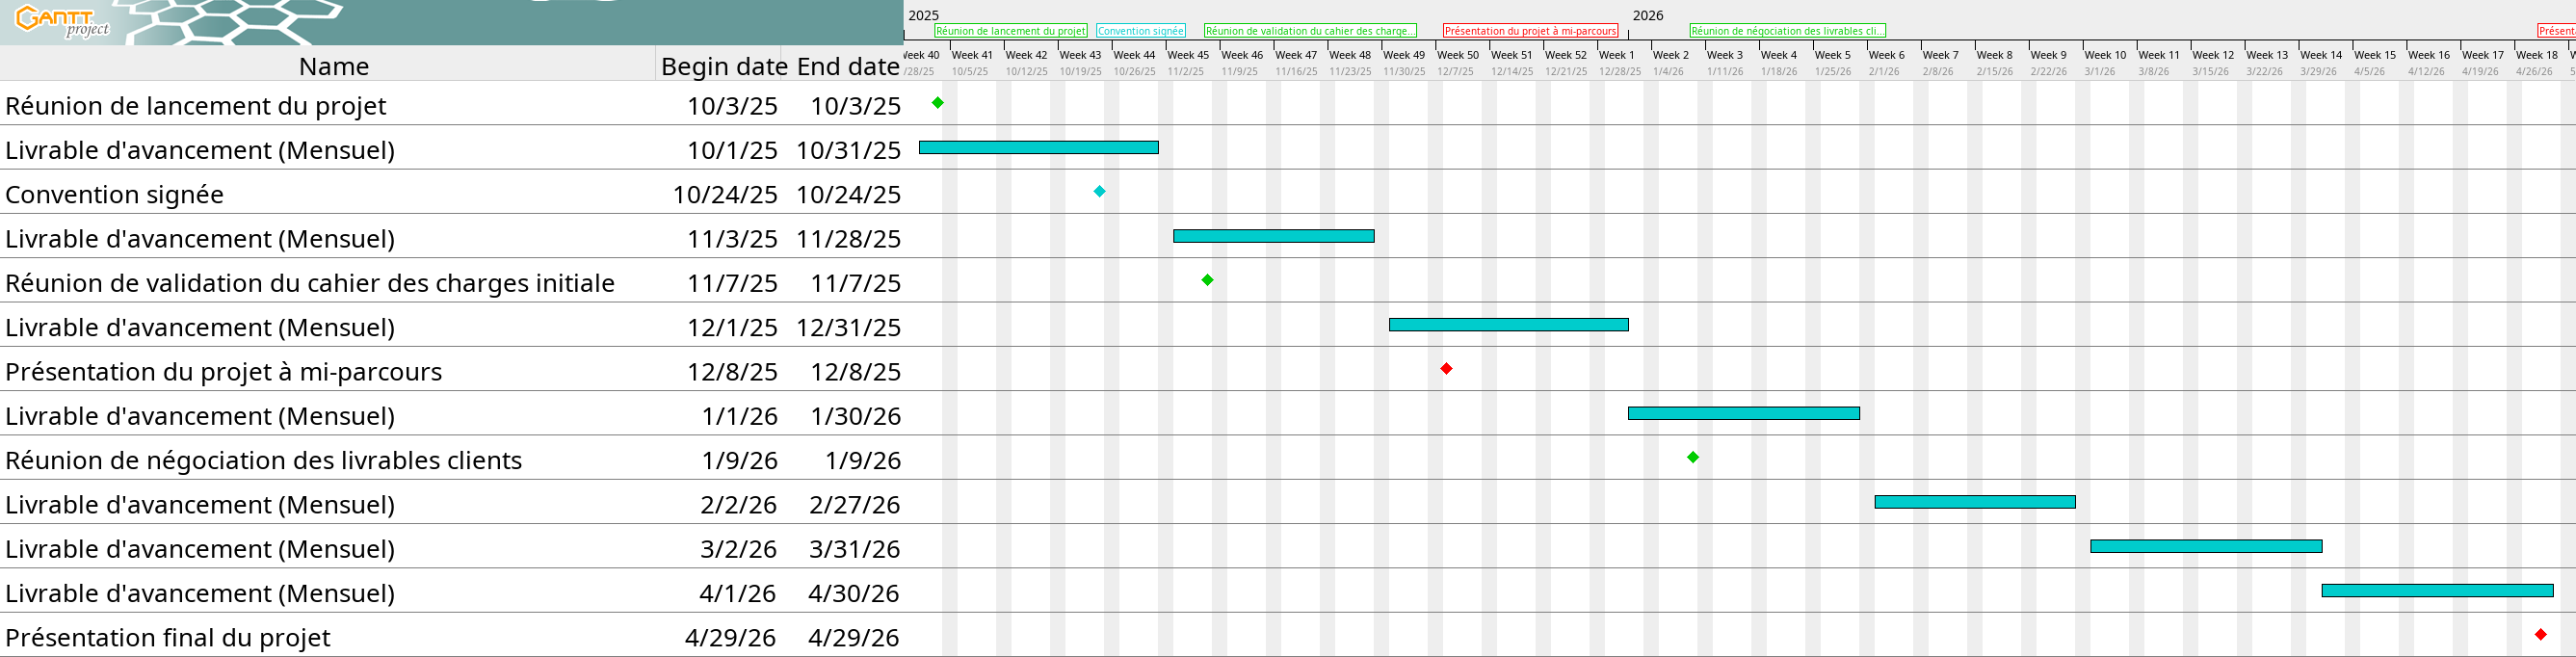
\includegraphics[width=1\textwidth]{images/livrables_avancer_projet_client.png}
   }
   \caption{Gantt des livrables de négociation et de suivi d’avancement du projet}
   \label{fig:LivClient}
\end{figure}
\vspace{1em}

Un rapport mensuel sera remis au client afin de suivre l'avancement du projet. La fréquence de remise de ce rapport pourra évoluer au cours du projet selon les demandes du client.
\newline

À l’issue du projet, un piège caméra capable de détecter les mouvements d’animaux, de capturer des photos et d’envoyer les données vers un stockage distant, sera à remettre au client.\newline

\vspace{1cm}
Le diagramme de Gantt ci-dessous permet de visualiser les livrables, produits à rendre au clients.
\begin{figure}[h]
   \centering
   {
      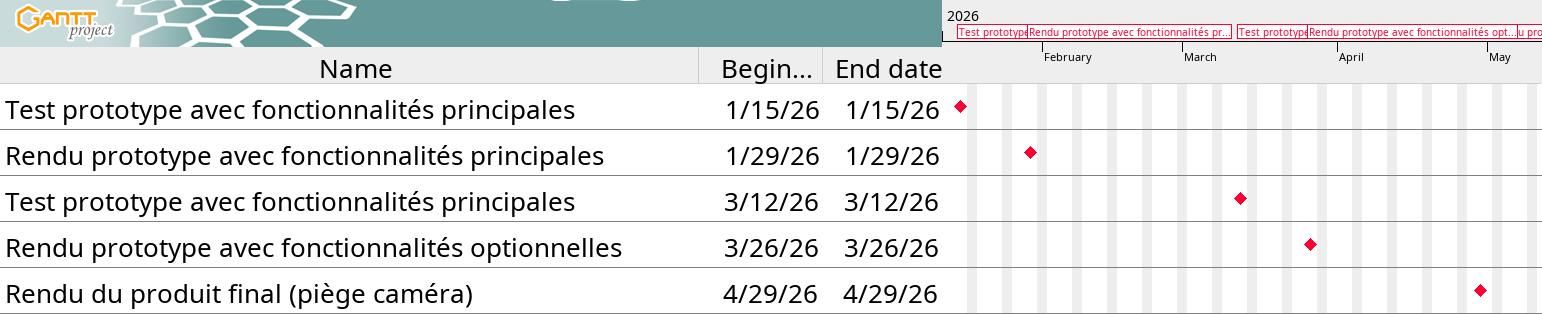
\includegraphics[width=1\textwidth]{images/Livrables_produits_client.png}
   }
   \caption{Diagramme de Gantt des livrables produits pour le client}
   \label{fig:LivClient}
\end{figure}
\vspace{1em}

% \vspace{2em}
% Le diagramme de Gantt ci-dessous permet de visualiser l'ensemble des tâches de chaques work packages des fonctions principales du projets. Une couleur représente un work package. \\
% \begin{figure}[h]
%    \hspace{-1cm}
%    {
%       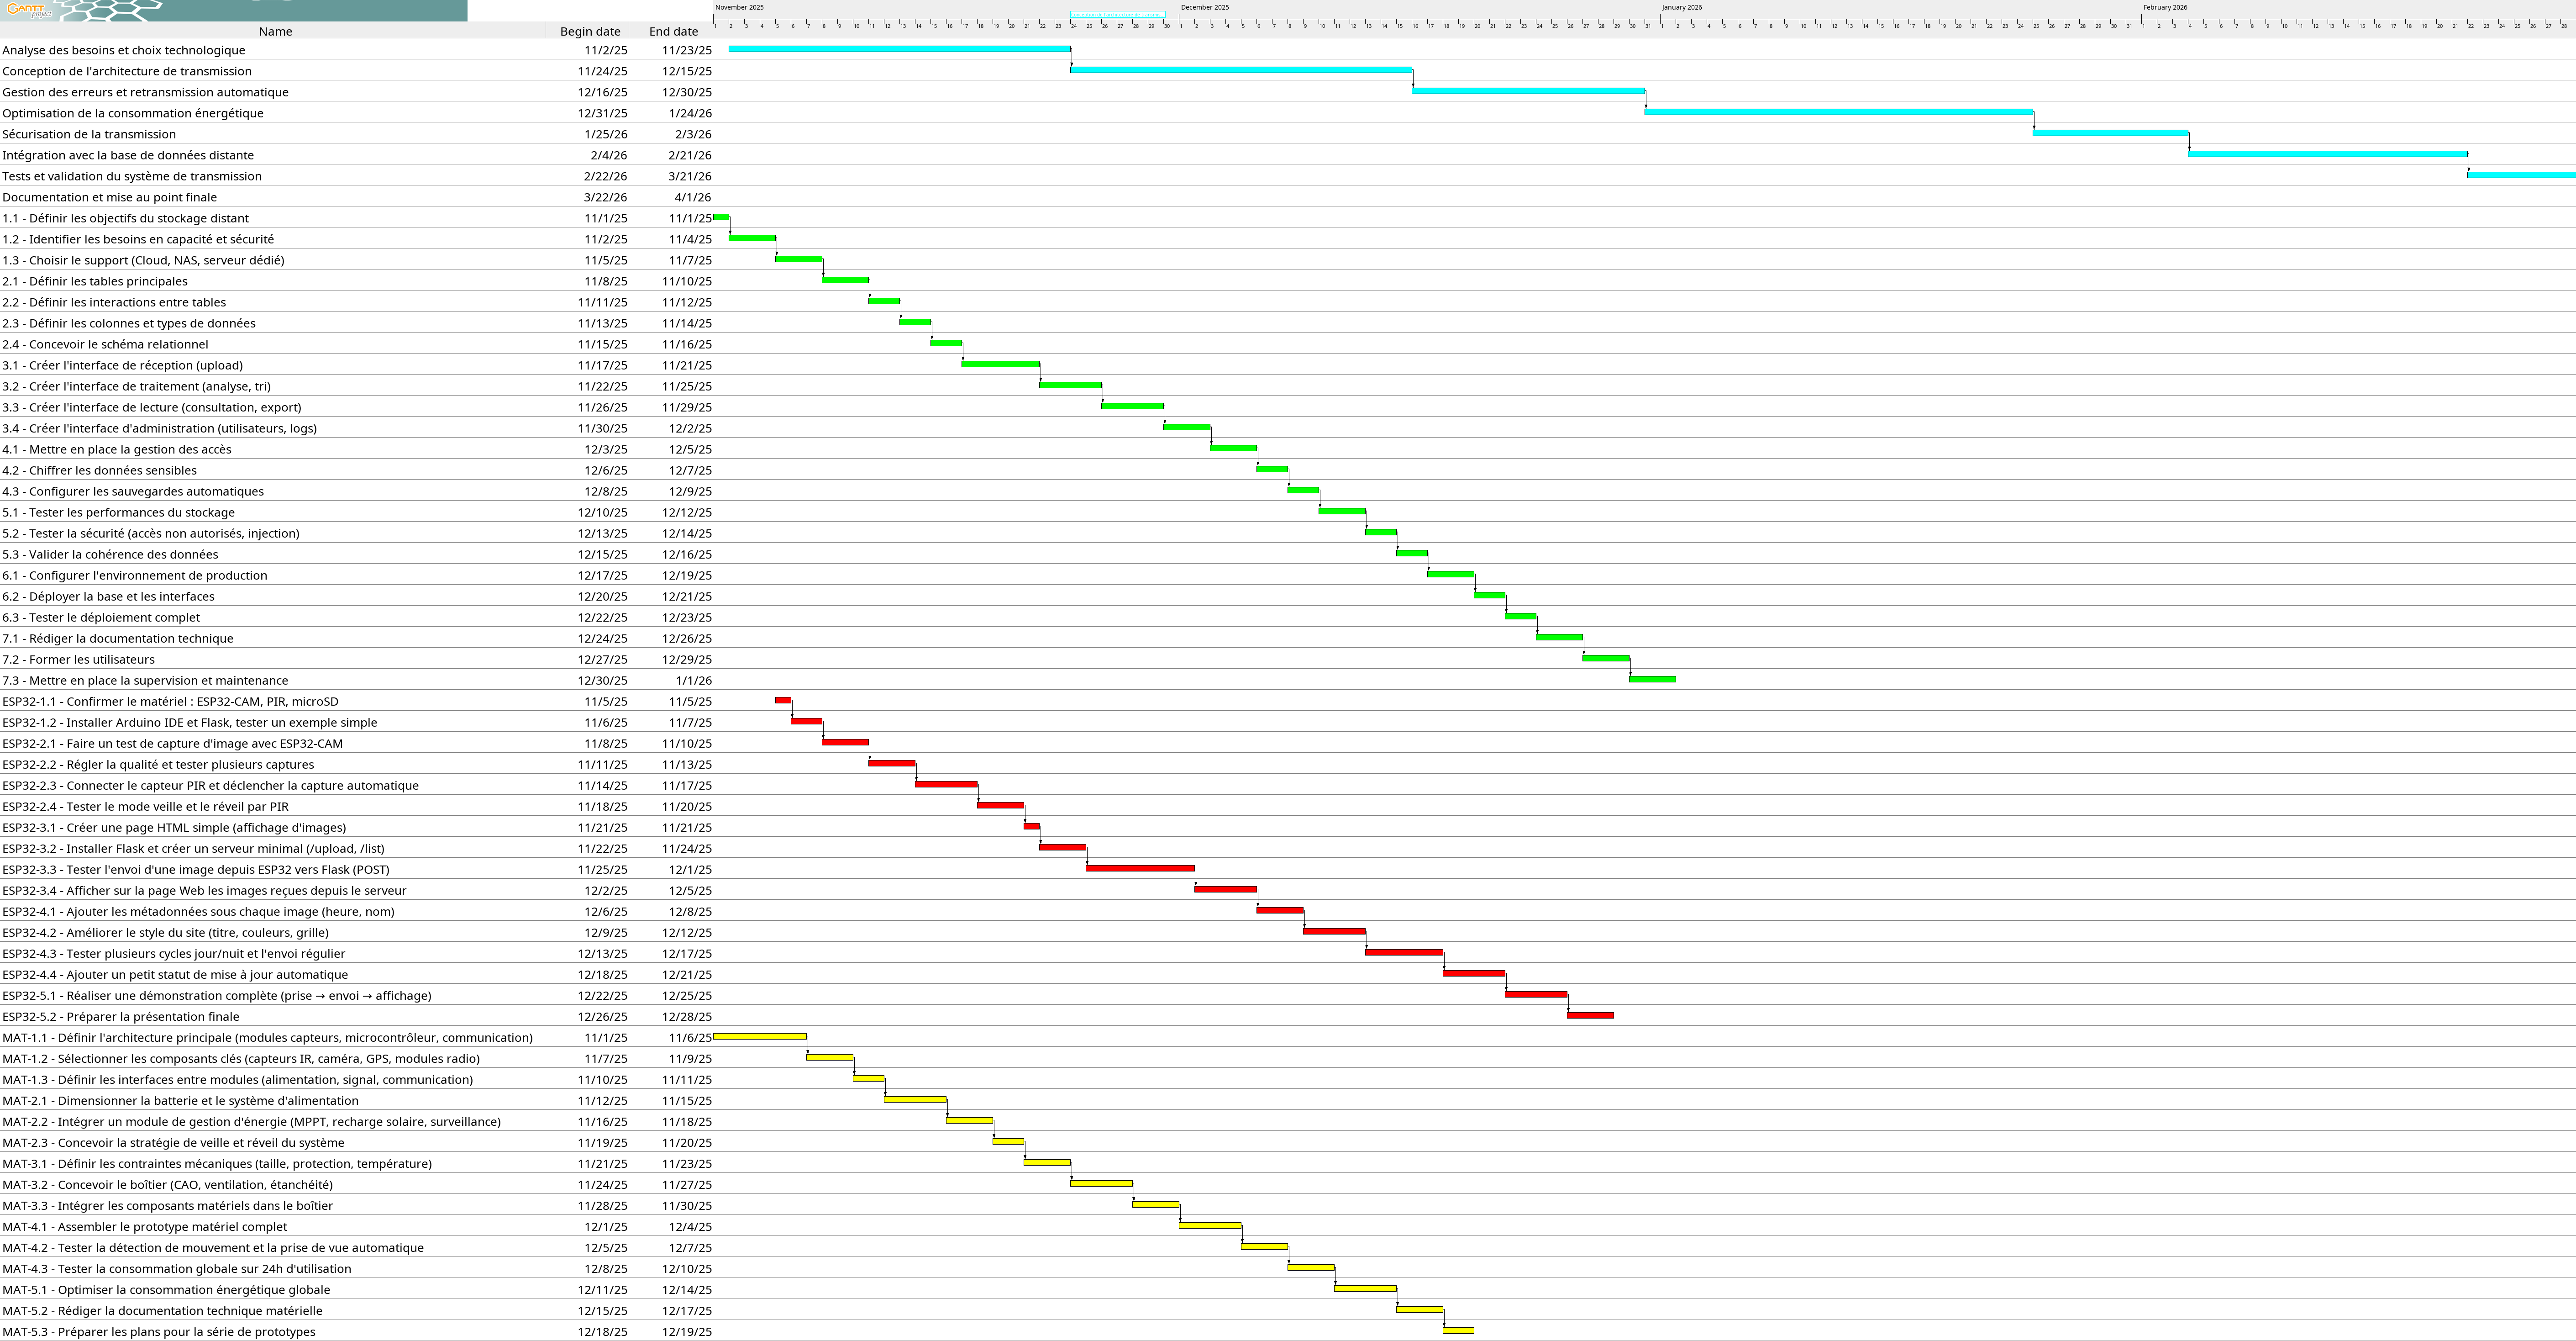
\includegraphics[width=1.1\textwidth]{images/Gantt_taches_wp.png}
%    }
%    \caption{Diagramme de Gantt des livrables produits pour le client}
%    \label{fig:LivClient}
% \end{figure}